%=======================================================================
%  BIL 401 — Interim Status Report
%  Derleme:  pdflatex main  ->  bibtex yok (refs gomulu)  ->  pdflatex main x2
%  Gerekli:  figures/ klasoru main.tex ile ayni dizinde olmali
%=======================================================================
\documentclass[conference]{IEEEtran}
\IEEEoverrideabstractsetup

\usepackage{graphicx}
\usepackage{amsmath,amssymb}
\usepackage{booktabs}
\usepackage{url}
\usepackage[hidelinks]{hyperref}
\usepackage{xcolor}

\graphicspath{{figures/}}

\begin{document}

\title{Freshness, Not Policy: Re-evaluating Adaptive GNN\\
Embedding Updates on the Elliptic Bitcoin Graph}

\author{
\IEEEauthorblockN{Mithat Dursun \quad Muhittin Berke Bilgin}
\IEEEauthorblockA{221101037 \quad\quad 221401027\\
\texttt{m.dursun@etu.edu.tr}}
}

\maketitle

%=======================================================================
\begin{abstract}
This interim report re-evaluates embedding-refresh policies for a graph neural
network operating on a streaming transaction graph. The system combines the
Elliptic Bitcoin dataset, Apache Kafka, PySpark Structured Streaming, a
previously trained GraphSAGE model and a Docker-based distributed execution
layer with two Spark workers. Five policies are compared: NoRefresh,
FullAlways, LocalAlways, LocalPeriodic and LocalAdaptive, the last under a
threshold sweep $\tau \in \{0.05, 0.15, 0.25, 0.35, 0.50\}$. All quality results
are obtained from a matched replay protocol and repeated over three
independently trained models.
The central result is methodological. Absolute test AUPRC is not stable: it
varies by $17.7\%$ across seeds ($0.4210 \pm 0.0746$) while validation AUPRC
varies by only $1.0\%$, a variance ratio of $7.8$, so early stopping on
validation does not control test-period performance. Relative structure, by
contrast, is highly stable: the correlation between fresh-at-arrival rate and
arrival-time AUPRC is $\rho = -0.844 \pm 0.010$, and all five pairwise policy
contrasts preserve their sign in all three seeds. LocalPeriodic falls on the
same freshness--quality trend as the LocalAdaptive sweep despite a different
selection rule, indicating that the controlling variable is the level of
staleness rather than the policy producing it.
A never-refreshed control outperforms full refresh by $0.1432 \pm 0.0622$
AUPRC. An edge ablation explains why: removing all edges improves AUPRC in
$23$ of $24$ pre-drift time-step comparisons, with a mean gain of $0.155$. Two
independent code paths agree exactly on this control, and the mechanism is
visible in the data, since the graph has mean degree $2.30$ and the
neighbourhood label purity of illicit nodes falls from $0.518$ in training to
$0.265$ after the regime change at time step $43$. Finally, node-update count
is shown to be an insufficient cost proxy: LocalAdaptive performs $2.6\times$
fewer updates than LocalAlways yet exhibits $2.3\times$ worse tail latency.
We therefore report differences rather than levels and do not declare a
winning policy at this stage.
\end{abstract}

\begin{IEEEkeywords}
graph neural networks, streaming graphs, node embeddings, Apache Kafka,
PySpark Structured Streaming, Docker, concept drift, adaptive updates
\end{IEEEkeywords}

%=======================================================================
\section{Introduction}

The objective of this project is to study how node embeddings produced by a
graph neural network (GNN) can be updated efficiently when graph data arrives
continuously. In a static workflow the graph is assumed fixed while embeddings
are computed. In the streaming setting considered here, new transaction
relationships arrive over time and alter the neighbourhoods of existing nodes,
so previously computed embeddings may become stale.

Recomputing every node after each incoming batch is a direct reference
solution, but its cost grows rapidly with graph size. The project therefore
compares full-graph, local, periodic and adaptive update strategies, together
with a never-refreshed control that isolates the contribution of refresh
itself.

The previous status report presented a single-run comparison and concluded that
the adaptive policy achieved the best arrival-time quality. This report
withdraws that conclusion. Three developments are responsible. First, a
dedicated NoRefresh baseline shows that the high arrival-time scores previously
attributed to selective refresh are obtainable with no refresh at all. Second,
repeating the experiment over three training seeds shows that absolute scores
are not stable enough to support a single-run ranking. Third, an edge ablation
identifies the mechanism, which turns out to be a structural property of the
graph rather than a consequence of the temporal drift. The report is therefore
organised around what is measurable and reproducible rather than around a
proposed winner.

%=======================================================================
\section{Dataset and Preprocessing}

The Elliptic dataset provides a labelled Bitcoin transaction graph
\cite{weber2019}. The preprocessing pipeline maps transaction identifiers to
graph-node indices and produces a node-feature matrix, an edge index, a label
mapping and a chronological stream file for Kafka ingestion.
Table~\ref{tab:data} summarises the resulting structures.

\begin{table}[t]
\centering
\caption{Processed dataset.}
\label{tab:data}
\small
\begin{tabular}{@{}lr@{}}
\toprule
Quantity & Value \\
\midrule
Nodes & 203{,}769 \\
Directed edges & 234{,}355 \\
Undirected edges (symmetrised) & 468{,}710 \\
Node features & 165 \\
Labelled nodes & 46{,}564 \\
\quad illicit / licit & 4{,}545 / 42{,}019 \\
Unlabelled nodes & 157{,}205 \\
\midrule
Train (ts $1$--$29$), labelled & 26{,}381 \\
Validation (ts $30$--$34$), labelled & 3{,}513 \\
Test (ts $35$--$49$), labelled & 16{,}670 \\
\bottomrule
\end{tabular}
\end{table}

Three design decisions follow the standard temporal protocol. The time step is
not supplied as a feature, to avoid temporal leakage. Feature standardisation
uses training-period statistics only. Every forward pass is restricted to edges
whose endpoints lie within the corresponding period, which is enforced by an
explicit filter even though Elliptic edges already fall within a single time
step.

The raw edge list is directed and contains no reciprocal pairs, so
symmetrisation is not optional; both the offline pipeline and the streaming
graph store insert each edge in both directions.

%=======================================================================
\section{System Architecture}

Kafka is the transport layer for graph-update records and PySpark Structured
Streaming provides the micro-batch interface. Execution is distributed across
two Dockerised Spark workers, each running the GNN application through a
\texttt{spark-runner} container. Table~\ref{tab:platform} lists component
status.

An earlier Java compatibility problem is retained for completeness: Java 23
caused startup failures with the selected Spark/PySpark environment, and
Java 17 was installed and selected instead. This established the compatible
runtime used by all subsequent work.

\begin{table}[t]
\centering
\small
\caption{Platform and component status.}
\label{tab:platform}
\begin{tabular}{@{}p{2.4cm}p{3.4cm}l@{}}
\toprule
Component & Purpose & Status \\
\midrule
Apache Kafka & buffers update records & operational \\
Spark Streaming & forms micro-batches & operational \\
Docker runtime & isolates services & operational \\
\texttt{spark-worker1/2} & partitioned processing & operational \\
\texttt{gnn-app} + runner & worker-side GNN execution & integrated \\
Pretrained GraphSAGE & parameters, initial embeddings & integrated \\
\bottomrule
\end{tabular}
\end{table}

The refresh engine is deliberately independent of the source of a micro-batch.
The same \texttt{GraphStore}, \texttt{EmbeddingStore} and policy classes are
driven either by the Kafka consumer or by a static replay driver, which is what
makes the two evaluation paths in Section~\ref{sec:consistency} comparable.

%=======================================================================
\section{Refresh Policies}

Let $V_t$ denote the node set after batch $t$, let $A_t^{(L)}$ be the nodes
affected by the batch expanded to an $L$-hop neighbourhood, and let $s_t(v)$ be
the staleness score of node $v$. The update set $U_t$ is

\begin{equation}
U_t =
\begin{cases}
\varnothing, & \text{NoRefresh},\\[2pt]
V_t, & \text{FullAlways},\\[2pt]
A_t^{(L)}, & \text{LocalAlways},\\[2pt]
\bigcup_{i=t-N+1}^{t} A_i^{(L)}, & \text{LocalPeriodic},\\[2pt]
\{v \in A_t^{(L)} : s_t(v) > \tau\}, & \text{LocalAdaptive}.
\end{cases}
\end{equation}

The staleness score combines three normalised components,
\begin{equation}
s_t(v)=\alpha\,n(\Delta t_v)+\beta\,n(\Delta d_v)+\gamma\,n(\Delta c_v),
\end{equation}
where $\Delta t_v$ is the time since $v$ was last refreshed, $\Delta d_v$ the
degree change and $\Delta c_v$ the number of neighbours refreshed since, and
$n(x)=1-e^{-x/\sigma}$ is a bounded normaliser. Throughout we use
$\alpha=0.5$, $\beta=\gamma=0.25$ and $N=5$.

NoRefresh is the control arm. It keeps the entire refresh loop --- graph
insertion, affected-set computation and prediction --- and changes only the
selection decision, so any difference against the other policies is
attributable to refresh alone.

%=======================================================================
\section{Experimental Protocol}
\label{sec:protocol}

All quality results use one replay protocol: 60 micro-batches, four batches per
time step over the test period, 16{,}670 predictions, zero fallback
predictions, and a decision threshold selected on the validation split. A node
is scored at the moment it first appears in the stream, using whatever
embedding the cache currently holds; this is the arrival-time metric. A
secondary end-of-stream metric rescores all nodes with the final cache.

The replay driver is deterministic. The model is evaluated with dropout
disabled, batch boundaries are fixed, and no sampling is involved. Changing the
replay seed therefore changes nothing, and the fresh-at-arrival rate of every
policy has zero variance across runs. The only stochastic component of the
pipeline is training. Accordingly, the multi-seed experiment retrains the model
for each seed and then runs the full policy suite on each resulting model.

Quality metrics are not taken from the distributed Kafka runs. In those runs
the first micro-batch drained the entire topic, so the graph was already
complete when the first predictions were emitted; the signature is that
FullAlways reports identical arrival-time and end-of-stream AUPRC there,
whereas under incremental replay the two differ. The distributed runs are
retained for throughput and latency diagnostics only.

%=======================================================================
\section{Results}

\subsection{Stability: levels are unreliable, rankings are not}
\label{sec:multiseed}

Training was repeated with three seeds. Validation AUPRC is stable at
$0.9418 \pm 0.0096$, a coefficient of variation of $1.0\%$. Test AUPRC for the
same configuration is not: $0.4210 \pm 0.0746$, a coefficient of variation of
$17.7\%$ and a variance ratio of $7.8$ against validation. The selected
decision threshold likewise moves, at $0.9062 \pm 0.0095$. Model selection and
early stopping on validation AUPRC therefore do not control test-period
performance in this setting, and single-run absolute scores should not be
reported as headline results.

Because all policies within a seed share one trained model, policy comparisons
are paired and are unaffected by this level shift.
Figure~\ref{fig:multiseed} shows both facts: the freshness--quality curve keeps
its shape while its level moves by up to $0.14$ AUPRC, and every pairwise
contrast preserves its sign in all three seeds.
Table~\ref{tab:paired} lists the contrasts.

\begin{figure*}[t]
\centering
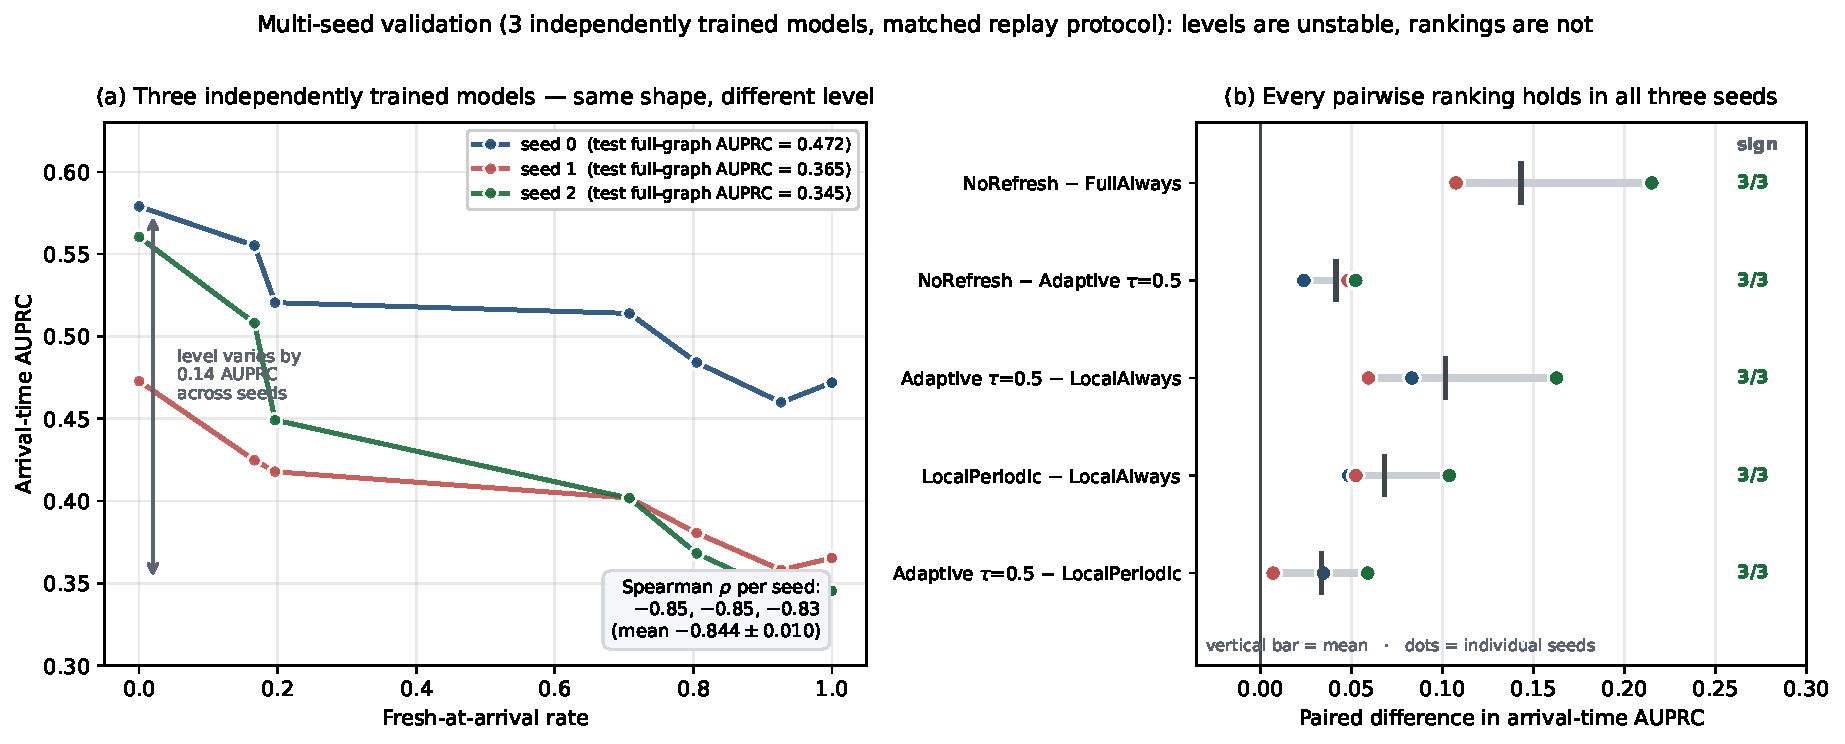
\includegraphics[width=\textwidth]{multiseed_paired.pdf}
\caption{Multi-seed validation over three independently trained models.
(a) The freshness--quality curve keeps its shape while its level shifts across
seeds. (b) Every pairwise ranking holds in all three seeds; dots are individual
seeds and the vertical bar is the mean.}
\label{fig:multiseed}
\end{figure*}

\begin{table}[t]
\centering
\small
\caption{Paired differences in arrival-time AUPRC across three seeds. Because
policies within a seed share a model, these contrasts are unaffected by the
seed-level shift. ``Adaptive'' denotes LocalAdaptive at $\tau{=}0.50$.}
\label{tab:paired}
\begin{tabular}{@{}lrc@{}}
\toprule
Contrast & Mean $\pm$ s.d. & Sign \\
\midrule
NoRefresh $-$ FullAlways      & $+0.1432 \pm 0.0622$ & 3/3 \\
NoRefresh $-$ Adaptive        & $+0.0414 \pm 0.0154$ & 3/3 \\
Adaptive $-$ LocalAlways      & $+0.1018 \pm 0.0541$ & 3/3 \\
LocalPeriodic $-$ LocalAlways & $+0.0683 \pm 0.0308$ & 3/3 \\
Adaptive $-$ LocalPeriodic    & $+0.0335 \pm 0.0260$ & 3/3 \\
\bottomrule
\end{tabular}
\end{table}

\subsection{Freshness governs arrival-time quality}

Table~\ref{tab:main} reports all nine configurations. Across them, the
fresh-at-arrival rate and arrival-time AUPRC are strongly negatively
correlated, with a per-seed Spearman coefficient of $-0.85$, $-0.85$ and
$-0.83$, that is $\rho = -0.844 \pm 0.010$. This is the most stable quantity
measured in the study.

Two observations follow. First, LocalPeriodic lies on the same trend as the
LocalAdaptive sweep despite using a completely different selection rule. Within
this experiment the controlling variable is therefore not the identity of the
policy but the level of freshness it produces; a policy acts as a dial on
staleness rather than as an independent mechanism.

Second, the end-of-stream column behaves differently from the arrival-time
column. Every fully refreshed configuration converges to the same value and the
never-refreshed control is highest, while all partially refreshed
configurations fall strictly between the two extremes and decline monotonically
as the cache becomes more mixed. The penalty is small but it is the most
reproducible effect we measured: FullAlways exceeds LocalAdaptive
$\tau{=}0.50$ by $0.0065 \pm 0.0008$ AUPRC at end of stream, an effect eight
times its own standard deviation, with the same sign in all three seeds. A
cache that mixes rows computed under different graph states is thus worse than
either homogeneous extreme.

\begin{table*}[t]
\centering
\caption{All policies over three independently trained models under the matched
replay protocol of Section~\ref{sec:protocol}. Quality values are mean $\pm$
s.d.\ across seeds. Node updates and fresh rate are deterministic functions of
the graph and policy, so they carry no seed variance.}
\label{tab:main}
\small
\begin{tabular}{@{}lrrrrr@{}}
\toprule
Policy & Fresh rate & Arrival AUPRC & EOS AUPRC & Node updates & Wall p99 (ms) \\
\midrule
NoRefresh (control)             & 0.000 & $\mathbf{0.5375 \pm 0.0567}$ & $\mathbf{0.5375 \pm 0.0567}$ & 0 & $13.5 \pm 0.1$ \\
FullAlways                      & 1.000 & $0.3943 \pm 0.0680$ & $0.4210 \pm 0.0746$ & 12{,}226{,}140 & $228.1 \pm 6.5$ \\
LocalAlways                     & 1.000 & $0.3943 \pm 0.0680$ & $0.4210 \pm 0.0746$ & 178{,}883 & $23.6 \pm 0.8$ \\
LocalPeriodic $N{=}5$           & 0.196 & $0.4625 \pm 0.0526$ & $0.4210 \pm 0.0746$ & 92{,}923 & $28.8 \pm 0.8$ \\
LocalAdaptive $\tau{=}0.05$     & 1.000 & $0.3943 \pm 0.0680$ & $0.4209 \pm 0.0746$ & 152{,}649 & $25.6 \pm 1.3$ \\
LocalAdaptive $\tau{=}0.15$     & 0.927 & $0.3876 \pm 0.0631$ & $0.4198 \pm 0.0743$ & 125{,}226 & $29.6 \pm 0.4$ \\
LocalAdaptive $\tau{=}0.25$     & 0.805 & $0.4110 \pm 0.0637$ & $0.4189 \pm 0.0745$ & 112{,}439 & $32.0 \pm 2.2$ \\
LocalAdaptive $\tau{=}0.35$     & 0.708 & $0.4392 \pm 0.0648$ & $0.4162 \pm 0.0743$ & 98{,}723 & $34.8 \pm 0.3$ \\
LocalAdaptive $\tau{=}0.50$     & 0.167 & $0.4960 \pm 0.0660$ & $0.4144 \pm 0.0738$ & 69{,}641 & $54.1 \pm 0.4$ \\
\bottomrule
\end{tabular}
\end{table*}

\subsection{Internal consistency}
\label{sec:consistency}

Four checks support the measurement pipeline, and all four hold in every seed.
FullAlways and LocalAlways agree to four decimals on both metrics, confirming
that restricting recomputation to the $L$-hop affected set is lossless.
LocalAdaptive at $\tau{=}0.05$ reproduces the FullAlways operating point
exactly, so the sweep is anchored correctly. Most importantly, two independent
code paths agree: the offline edge ablation with an empty edge set returns
exactly the arrival-time AUPRC that the streaming replay reports for NoRefresh,
and the ablation with the complete graph returns exactly the end-of-stream
AUPRC that the replay reports for FullAlways. The streaming engine and the
offline evaluator therefore measure the same quantities.

\subsection{Why the never-refreshed control wins}

An edge ablation isolates the contribution of neighbourhood aggregation.
Evaluating the same trained encoder with the complete graph and with an empty
edge set gives a gain of $+0.0723$, $+0.0883$ and $+0.1889$ AUPRC for the three
seeds, all positive.

Figure~\ref{fig:ablation} locates the effect in time. The no-edge variant wins
in $23$ of the $24$ pre-drift time-step comparisons, with a mean gain of
$+0.155$ AUPRC. After the regime change at time step $43$ both variants fall
close to the class prior and the remaining differences are not interpretable.
Since $84\%$ of the labelled illicit test nodes occur before time step $43$,
the aggregate effect is driven by the pre-drift period. \emph{The advantage of
stale embeddings is therefore a structural property of this graph rather than a
consequence of the drift.} The drift is a separate and more destructive
phenomenon that removes the discriminative power of both variants.

\begin{figure}[t]
\centering
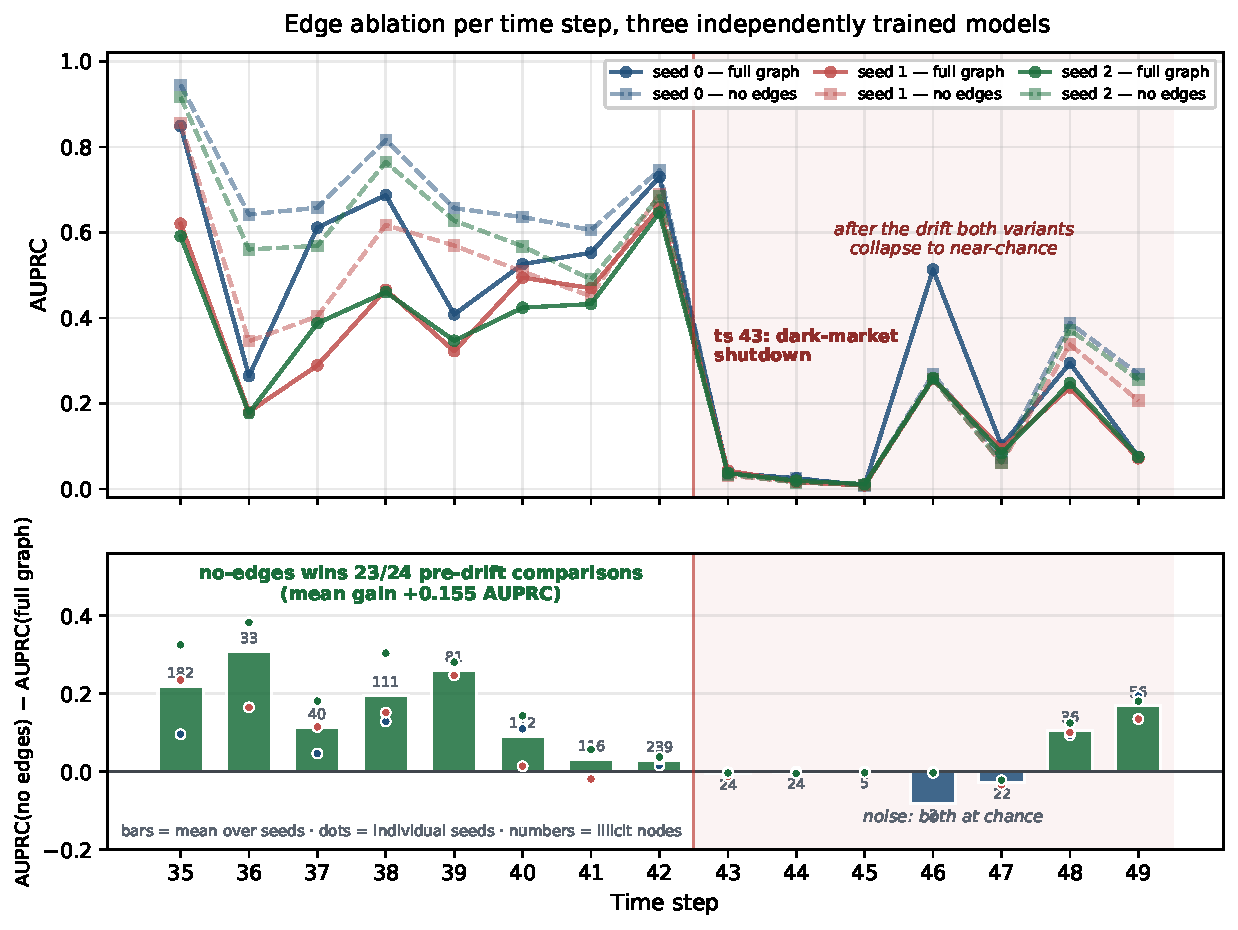
\includegraphics[width=\columnwidth]{edge_ablation_by_ts.pdf}
\caption{Edge ablation per test time step over three trained models. Removing
all edges improves AUPRC in almost every pre-drift time step; after the regime
change at time step 43 both variants approach chance.}
\label{fig:ablation}
\end{figure}

Three properties of the data explain the result, and none require running the
model. They are summarised in Figure~\ref{fig:mechanism}.

First, the neighbourhood label signal drifts. For an illicit node, the fraction
of its labelled neighbours that are themselves illicit is $0.518$ over the
training period, $0.413$ over test time steps $35$--$42$ and only $0.265$ after
time step $43$. The aggregation weights were fitted under the first regime and
are applied under the third, so for the positive class the neighbourhood term
becomes actively misleading: a post-drift illicit node has on average roughly
three licit neighbours for every illicit one, and mean aggregation pulls its
representation towards the licit region.

Second, the graph is very sparse. The mean undirected degree is $2.30$, the
median is $2$, and $76\%$ of labelled test nodes have at most two neighbours;
the median two-hop neighbourhood contains six nodes. For a large fraction of
nodes, mean aggregation is an average over a single neighbour, which
contributes variance rather than information. A further $25.6\%$ of labelled
test nodes have no labelled neighbour at all.

Third, degree itself carries signal that the aggregator discards. Illicit rates
are $9.9\%$, $5.5\%$ and $2.0\%$ for test nodes of degree one, two and at least
three, yet the mean aggregator is degree-invariant by construction. The initial
embeddings avoid all three problems, because they were computed without
test-period edges and therefore reduce to the feature-only path, which already
contains the aggregated neighbourhood statistics supplied with the dataset and
computed over the complete static graph.

\begin{figure*}[t]
\centering
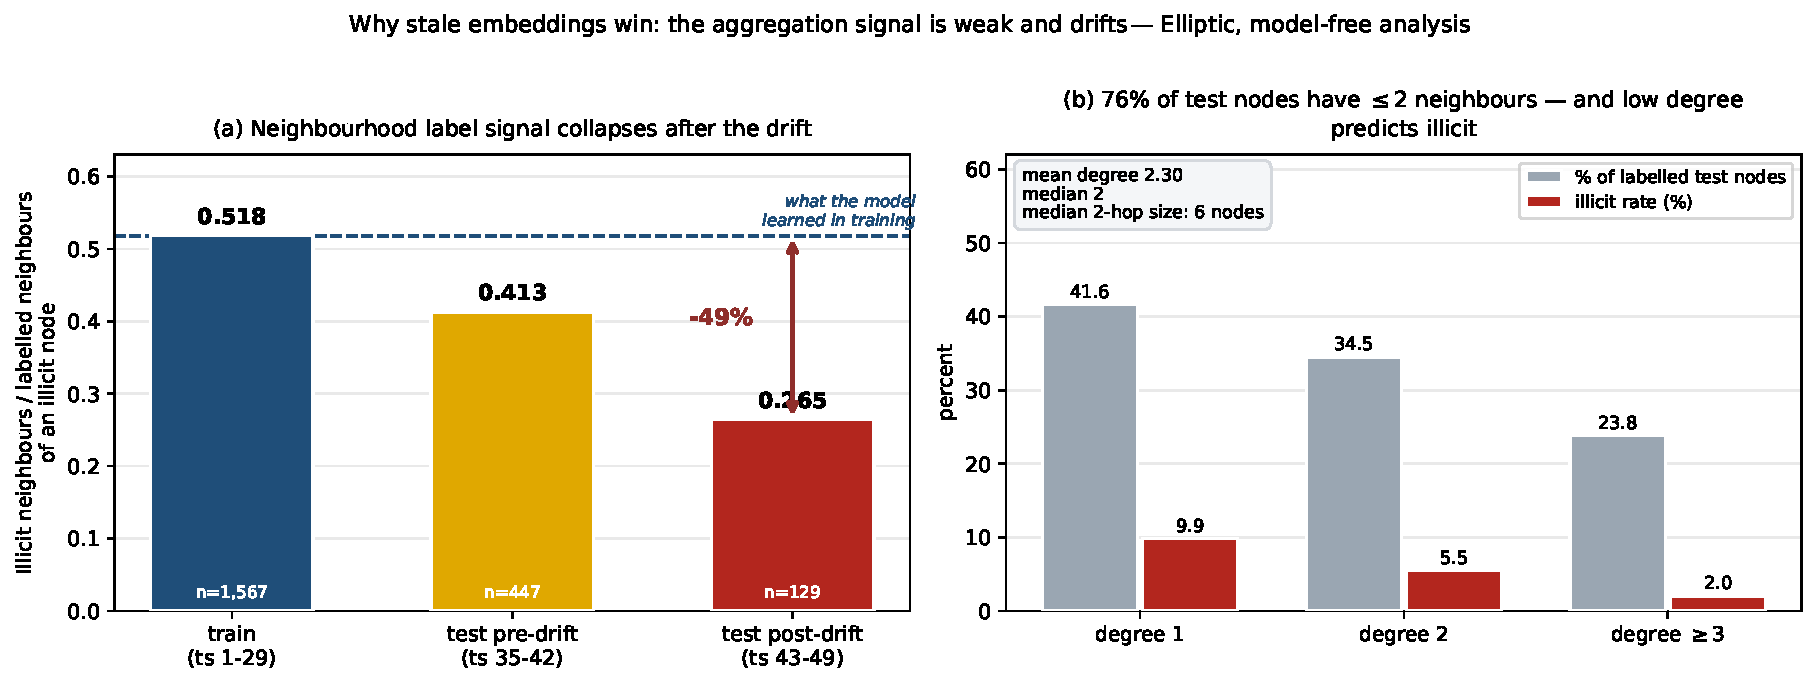
\includegraphics[width=\textwidth]{why_stale_wins.pdf}
\caption{Model-free analysis. (a) The fraction of an illicit node's labelled
neighbours that are themselves illicit falls sharply after the regime change.
(b) The graph is extremely sparse and low degree is itself predictive of the
illicit class.}
\label{fig:mechanism}
\end{figure*}

\subsection{Node-update count is an insufficient cost proxy}

NoRefresh performs no embedding refresh at all yet still incurs a p99 batch
wall time of $13.5$~ms. This is the cost of maintaining the graph state and
computing affected sets, and it forms a floor for every policy. Against that
floor, LocalAlways adds $10.1$~ms for $178{,}883$ updates, whereas
LocalAdaptive at $\tau{=}0.50$ adds $40.6$~ms for only $69{,}641$ updates. The
proposed adaptive policy therefore performs $2.6\times$ fewer node updates than
LocalAlways while exhibiting $2.3\times$ worse tail latency
(Figure~\ref{fig:cost}).

Two effects plausibly contribute. The staleness pool is rescored on every
batch, and sparse adaptive targets are scattered across the graph so that each
selected set induces a comparatively large two-hop subgraph. Distinguishing
them requires instrumenting the number of nodes actually materialised for
refresh, which the current per-batch metrics do not record.

\begin{figure}[t]
\centering
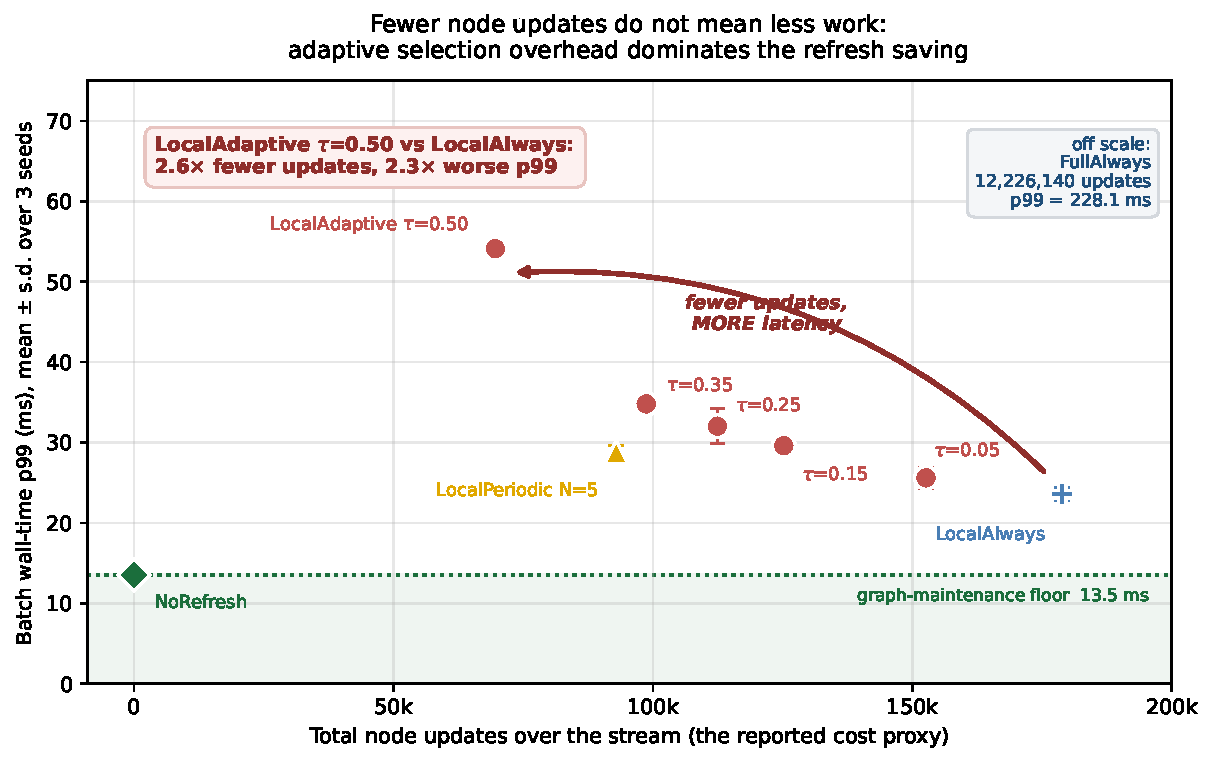
\includegraphics[width=\columnwidth]{cost_paradox.pdf}
\caption{Node-update count does not predict work. LocalAdaptive performs fewer
updates than LocalAlways yet shows substantially higher tail latency. Error
bars are one standard deviation over three seeds.}
\label{fig:cost}
\end{figure}

\subsection{Two metric caveats}

\subsubsection{AUPRC is not comparable across splits}
The apparent fall from a validation AUPRC of $0.9418$ to a test AUPRC of
$0.4210$ should not be read as a collapse in model quality. AUPRC is bounded
below by the positive-class prior, and that prior falls from $0.1682$ on
validation to $0.0650$ on test and to $0.0253$ after time step $43$
(Table~\ref{tab:prior}). Normalising each score by its own baseline gives a
lift of $5.60\times$ on validation against $6.48\times$ for FullAlways and
$8.27\times$ for NoRefresh on test. Measured as separation above chance, the
model performs at least as well on the test period as on validation, and the
raw decline is largely an artefact of the shifting prior.

\begin{table}[t]
\centering
\caption{Class prior by temporal split. The AUPRC of a random classifier equals
the positive-class prior, so AUPRC is not comparable across splits without
normalisation.}
\label{tab:prior}
\begin{tabular}{lrrr}
\toprule
Split & Labelled & Illicit & Prior \\
\midrule
Validation (ts 30--34) & 3{,}513  & 591     & 0.1682 \\
Test (ts $\geq$ 35)    & 16{,}670 & 1{,}083 & 0.0650 \\
\quad ts 35--42        & 9{,}983  & 914     & 0.0916 \\
\quad ts 43--49        & 6{,}687  & 169     & 0.0253 \\
\bottomrule
\end{tabular}
\end{table}

\subsubsection{The decision threshold contains no leakage}
The threshold is selected by maximising $F_1$ on the validation split, using a
forward pass restricted to validation-period edges. Test data enters no step of
threshold selection. It is, however, calibrated on a pre-drift distribution,
which is why threshold-dependent metrics such as $F_1$ are less informative
here than AUPRC, and why the selected threshold itself varies across seeds.

%=======================================================================
\section{Related Work}

The project lies at the intersection of transaction-graph analysis, graph
representation learning and stream processing. The Elliptic dataset was
introduced for anti-money-laundering research on a labelled Bitcoin transaction
graph and has been evaluated with conventional classifiers and graph
convolutional models \cite{weber2019}. Graph convolutional networks combine
node attributes with information aggregated from neighbouring nodes
\cite{kipf2017}. GraphSAGE extends this through inductive neighbourhood
aggregation \cite{hamilton2017}.

Most standard GNN workflows assume a static graph during training or inference.
In a streaming graph, incoming edges change node neighbourhoods and invalidate
previously computed representations. Full recomputation is a useful baseline
but is costly; local methods restrict computation to affected neighbourhoods,
periodic methods reduce update frequency, and adaptive methods use a
state-dependent criterion. Kafka provides the distributed messaging layer
\cite{kreps2011} and Spark Structured Streaming the micro-batch interface
\cite{armbrust2018}.

Our finding that aggregation is a net negative in this regime is consistent
with the known difficulty of the post-shutdown Elliptic period reported in
\cite{weber2019}, but we locate the effect before rather than after that
regime change, and attribute it to graph sparsity and neighbourhood label
purity rather than to the drift itself.

%=======================================================================
\section{Next Steps}

The immediate next steps, in priority order, are as follows.

\begin{enumerate}
\item Record the number of nodes actually materialised for refresh, for example
      $|\mathrm{sub\_nodes}|$, and separate adaptive scoring time from subgraph
      construction and GNN forward time, so that the cost paradox of
      Figure~\ref{fig:cost} can be attributed rather than hypothesised.
\item Extend the seed study beyond three models and report confidence intervals
      rather than standard deviations, since several paired contrasts are
      consistent in sign but small relative to their spread.
\item Establish a matched end-to-end latency protocol by resetting the Kafka
      topic between runs, bounding records per trigger, and starting the
      consumer before the producer, so that timestamp-based latency becomes
      comparable across policies.
\item Test the sparsity hypothesis directly by replacing the mean aggregator,
      which is degree-invariant, with a degree-sensitive alternative, and by
      retraining on the local feature subset only, which removes the
      dataset-supplied aggregated statistics.
\item Extend sensitivity analysis to $\alpha$, $\beta$ and $\gamma$, and
      measure per-worker load balance and scaling beyond two workers.
\end{enumerate}

%=======================================================================
\section{Conclusion}

The project has progressed from a local Kafka--Spark prototype to a
Docker-based distributed architecture, and from a single-run policy comparison
to a matched, multi-seed evaluation with an explicit control arm.

The principal experimental finding is not that a particular refresh policy is
superior. It is that, under the present Elliptic replay and pretrained model,
arrival-time quality is governed by the level of embedding freshness rather
than by the policy that produces it, and that in this regime lower freshness is
associated with higher arrival-time quality. Across three independently trained
models the freshness--quality correlation is $\rho = -0.844 \pm 0.010$ and
every pairwise policy ranking preserves its sign, even though the absolute test
AUPRC of the same configuration varies by $17.7\%$ between seeds.

An edge ablation explains why stale embeddings are competitive: neighbourhood
aggregation is a net negative on this graph before the regime change, winning
in only one of twenty-four pre-drift comparisons, and the never-refreshed
control reduces exactly to the feature-only path. The adaptive policy
additionally fails to convert its smaller update count into lower latency.

We therefore report differences rather than levels, and we do not select a
winning policy or threshold at this stage. The measurements needed to do so
responsibly are listed as next steps.

%=======================================================================
\section*{Project Repository}
\url{https://github.com/Mithat07/Bil401_live_GNN_update}

%=======================================================================
\begin{thebibliography}{9}
\bibitem{weber2019}
M.~Weber \emph{et al.}, ``Anti-money laundering in Bitcoin: Experimenting with
graph convolutional networks for financial forensics,''
arXiv:1908.02591, 2019.

\bibitem{kipf2017}
T.~N.~Kipf and M.~Welling, ``Semi-supervised classification with graph
convolutional networks,'' in \emph{Proc. Int. Conf. Learn. Representations
(ICLR)}, 2017.

\bibitem{hamilton2017}
W.~L.~Hamilton, R.~Ying, and J.~Leskovec, ``Inductive representation learning
on large graphs,'' in \emph{Advances in Neural Information Processing Systems},
vol.~30, 2017.

\bibitem{kreps2011}
J.~Kreps, N.~Narkhede, and J.~Rao, ``Kafka: A distributed messaging system for
log processing,'' in \emph{Proc. NetDB}, 2011.

\bibitem{armbrust2018}
M.~Armbrust \emph{et al.}, ``Structured Streaming: A declarative API for
real-time applications in Apache Spark,'' in \emph{Proc. ACM SIGMOD Int. Conf.
Management of Data}, 2018, pp.~601--613.
\end{thebibliography}

\end{document}
